\chapter{Part-of-Speech (POS) Annotation Consistency}
\label{chap:pos-harmony}

We introduced the problem of inter treebank POS annotation quality in Section \ref{sec:harmony} earlier, followed by a discussion of the literature relevant to the problem in Section \ref{ssec:inconsistency-detection-pos}. 

In this chapter, we propose a metric based on $KL_{cpos^3}$ metric \citep{klcpos3}, which in turn is based upon Kullback-Liebler Divergence (KL Divergence). 

We start by a short introduction to $KL_{cpos^3}$ metric and a definition of the proposed metric in Section \ref{sec:pos-harmony-definition}. We define our dataset for the experiments in this chapter in Section \ref{sec:pos-harmony-dataset}, followed by the metric values being listed in Section \ref{sec:pos-harmony-scores}. The experiments are detailed in Section \ref{sec:pos-harmony-size} and Section \ref{sec:pos-harmony-genre}, with their results summarised in Section \ref{sec:pos-harmony-calculations}. The chapter concludes with a discussion on the metric in Section \ref{sec:pos-harmony-conclusion}.

\section{\texorpdfstring{$KL_{cpos^3}$}{KLcpos3} and Metric Definition}
\label{sec:pos-harmony-definition}

\cite{klcpos3} show that KL-Divergence score of POS trigrams can be effectively used for source selection for POS Tagging in a delexicalised cross-language model transfer scenario. In their approach, they are able to select effectively not just a singular source, but are also able to rank multiple sources by specifying weights to individual source in a multi-source transfer scenario. Computing the KL-Divergence on POS trigrams, they call the measure as $KL_{cpos^3}$, defined as follows:

\begin{definition}
\label{def:klcpos3}
\textbf{ }\\
\begin{equation}
\label{eqn:klcpos3}
\small KL_{cpos^3}(tgt, src) = \sum_{\forall cpos^3 \in tgt}^{}f_{tgt}(cpos^3)\log\frac{f_{tgt}(cpos^3)}{f_{src}(cpos^3)}
\end{equation}
where $cpos^3$ is a coarse POS tag trigram, and \\
\begin{align}
\label{eqn:cpos}
f(cpos^3) & = \nonumber f(cpos_{i-1}, cpos_{i}, cpos_{i+1}) \\ &= \frac{count(cpos_{i-1}, cpos_{i}, cpos_{i+1})}{\sum_{\forall cpos_{a,b,c}}{count(cpos_{a}, cpos_{b}, cpos_{c})}}
\end{align}
with $count_{src}(cpos^3) = 1$ for each unseen trigram.
\end{definition}

Intuitively, treebanks of the same language (despite the differences in the genres covered) should be better fit for single-source transfer than a treebank from another language. This is the primary motivation for using $KL_{cpos^3}$ (as defined for a single-source transfer scenario) to assess the annotation consistency among the treebanks of a language. However, $KL_{cpos^3}$ is a variant of KL-Divergence, and thus asymmetric, making it unfit in its original form for assessing annotation consistency symmetrically. We refer to the symmetric variant of the metric as $\theta_{pos}$ defined for the treebanks $A$ and $B$ as follows:

\begin{equation}
    \boxed{\theta_{pos}(A, B) = KL_{cpos^3}(A,B) + KL_{cpos^3}(B,A)}
\end{equation}
where $KL_{cpos^3}(P,Q)$ indicates $KL_{cpos^3}$ score of $Q$ as an estimator for $P$.

Since $KL_{cpos^3}$ is a non-negative divergence metric, so is $\theta_{pos}$. While either metric is numeric in nature, the $KL_{cpos^3}$ scores can be used as an estimator of quality in presence of an absolute gold standard. However, in absence of an absolute gold standard, the scores for the metric in different treebanks can not be compared directly. In such case (of lack of absolute gold standard), there should be an upper bound that needs to be placed on the $\theta_{pos}$ scores. As long as the $\theta_{pos}$ scores are lower than this upper bound, the considered pair of treebanks can be considered as harmonious in terms of their POS annotation. We call this upper bound as $\Theta_{pos}$. The metrics $\theta_{pos}$ and $\Theta_{pos}$ are linked together in the following definition.

\begin{definition}
\label{def:harmony}
Given two treebanks $A$ and $B$, we say the treebanks are in harmony with (or, are harmonious to) each other in terms of POS annotation, if the symmetric measure of their mutual divergence (given by $\theta_{pos}$) is less than or equal to a threshold (given by $\Theta_{pos}$). \\
    Mathematically, it can be represented as:
    \begin{align}
    \label{eq:pos_harmony}
        \Aboxed{\theta_{pos}(A, B) & = \nonumber KL_{cpos^3}(A,B) + KL_{cpos^3}(B,A)} \\
        &\leq \Theta_{pos}(A, B)
    \end{align}
    where $KL_{cpos^3}(P,Q)$ indicates $KL_{cpos^3}$ score of $Q$ as an estimator for $P$.
\end{definition}

Even though $\Theta_{pos}$ is a bound on the $\theta_{pos}$ metric, the former is essentially a property of the latter. For a given set of guidelines, and a given set of data, the upper bound value would need to be estimated often, albeit using the same technique. In the remaining chapter, we try to estimate the upper bound in a language-independent manner by looking at the influence of size of data, and the POS distribution in individual genres on $\theta_{pos}$ metric. While the methods that we shall discuss shortly can be applied for estimations across different guidelines and different set of data, care must be taken while estimating the upper bound for a new guideline (or even on different iterations of UD data). If the estimated value of $\Theta_{pos}$ is too large, we run the risk of saying the treebanks are harmonious even when they might not be. Also, if the value is too small, we could be overlooking at the effect of domain change and dataset size, to mistakenly announce the pair of treebanks as being non-harmonious to each other.

\section{Dataset}
\label{sec:pos-harmony-dataset}

UDv2.5 \citep{UDv2.5} contains 157 treebanks in 90 languages. There are multiple languages with more than one treebank, with some containing up to 6 treebanks. A list of all such languages, with the associated treebanks can be seen in Appendix \ref{app:multi_trees}. We list $\theta_{pos}$ scores of the different treebanks in different languages in the next section. In the listing of scores, the treebanks where the data needs to be fetched from another corpus because of licensing issues are not included.

As mentioned earlier, the treebanks in UD are assigned a score based on the system of checks run by the official UD validator. We want to estimate the $\Theta_{pos}$ scores to the best of our ability, and so, working with a pair of low quality treebanks would be the worst approach that can be undertaken. To that effect, we estimate the bounding score on treebanks with the ratings of at least 3.5 stars (out of 5 stars). The treebanks selected in this manner can be considered to be of high quality. The selection of high quality treebanks also enforces an important assumption, that the data within a singular treebank has been annotated consistently or that there are considerably lower number of annotation inconsistencies within the data in a treebank. The assumption would also imply that in a pair of considered treebanks, while the treebanks might not be annotated consistently with respect to each other, the individual treebanks are assumed to be internally consistent with respect to their annotation.

The assumption as mentioned above is a strict constraint, and might not always hold. An alternative assumption can be used in cases where the stricter version is not expected to hold. The relaxed version of the assumption assumes that the data belonging to one particular genre in a treebank would be annotated consistently throughout. This is a relaxation in the sense that given multiple genres in a treebank, the entire treebank might not be annotated consistently. However, the data in individual genres is annotated consistently. The experiments listed in this chapter work within the bound of these assumptions. 

\section{\texorpdfstring{$\theta_{pos}$}{theta\_pos} Scores for UDv2.5}
\label{sec:pos-harmony-scores}

\begin{minipage}{0.48\textwidth}
\subsection*{Languages with 2 Treebanks}
\begin{table}[H]
    \scalebox{0.90}{\begin{tabular}{|l|l|l|}
    \hline
    \textbf{Treebank1} & \textbf{Treebank2} & \textbf{$\theta_{pos}$} \\
    \hline
    \texttt{es}-AnCora & \texttt{es}-GSD & 0.352\\
    \hline
    \texttt{et}-EDT & \texttt{et}-EWT & 0.413 \\
    \hline
    \texttt{fi}-FTB & \texttt{fi}-TDT & 1.195 \\
    \hline
    \texttt{gl}-CTG & \texttt{gl}-TreeGal & 0.714 \\
    \hline
    \texttt{grc}-Perseus & \texttt{grc}-PROIEL & 4.641 \\
    \hline
    \texttt{ja}-GSD & \texttt{ja}-Modern & 2.915 \\
    \hline
    \texttt{ko}-GSD & \texttt{ko}-Kaist & 2.56 \\
    \hline
    \texttt{lt}-ALKSNIS & \texttt{lt}-HSE & 1.096 \\
    \hline
    \texttt{nl}-Alpino & \texttt{nl}-LassySmall & 0.664 \\
    \hline
    \texttt{orv}-RNC & \texttt{orv}-TOROT & 4.468 \\
    \hline
    \texttt{pl}-LFG & \texttt{pl}-PDB & 0.623 \\
    \hline
    \texttt{pt}-Bosque & \texttt{pt}-GSD & 0.678 \\
    \hline
    \texttt{sl}-SSJ & \texttt{sl}-SST & 2.405 \\
    \hline
    \texttt{sv}-LinES & \texttt{sv}-Talbanken & 0.443 \\
    \hline
    \texttt{tr}-GB & \texttt{tr}-IMST & 1.477 \\
    \hline
    \end{tabular}}
    \end{table}
    
    \subsection*{Languages with 4 Treebanks}
    
    \begin{table}[H]
    \scalebox{0.90}{\begin{tabular}{|l|l|l|l|}
    \hline
    \texttt{cs} & \textbf{CAC} & \textbf{CLTT} & \textbf{FicTree} \\
    \hline
    \textbf{CLTT} & 1.453 & - & - \\
    \hline
    \textbf{FicTree} & 1.138 & 2.657 & - \\
    \hline
    \textbf{PDT} & 0.373 & 1.935 & 1.006 \\
    \hline 
    \end{tabular}}
    \end{table}
    
    \vspace{1cm}
    \subsection*{Languages with 5 Treebanks}
    \end{minipage}
    \hfill
    \begin{minipage}{0.48\textwidth}
    \subsection*{Languages with 3 Treebanks}
    \begin{table}[H]
    \begin{tabular}{|l|l|l|}
    \hline
    \texttt{de} & \textbf{GSD} & \textbf{HDT} \\
    \hline
    \textbf{HDT} & 0.49 & - \\
    \hline
    \textbf{LIT} & 1.383 & 1.1 \\
    \hline
    \end{tabular}
    \end{table}
    
    \begin{table}[H]
    \begin{tabular}{|l|l|l|}
    \hline
    \texttt{la} & \textbf{ITTB} & \textbf{Perseus} \\
    \hline
    \textbf{Perseus} & 1.106 & - \\
    \hline
    \textbf{PROIEL} & 3.763 & 3.901 \\
    \hline
    \end{tabular}
    \end{table}
    
    \begin{table}[H]
    \scalebox{0.90}{\begin{tabular}{|l|l|l|}
    \hline
    \texttt{no} & \textbf{Bokmaal} & \textbf{Nynorsk} \\
    \hline
    \textbf{Nynorsk} & 0.095 & - \\
    \hline
    \textbf{NynorskLIA} & 2.291 & 2.375 \\
    \hline
    \end{tabular}}
    \end{table}
    
    \begin{table}[H]
    \scalebox{0.90}{\begin{tabular}{|l|l|l|}
    \hline
    \texttt{ro} & \textbf{Nonstandard} & \textbf{RRT} \\
    \hline
    \textbf{RRT} & 1.233 & - \\
    \hline
    \textbf{SiMoNERo} & 2.712 & 0.866 \\
    \hline
    \end{tabular}}
    \end{table}
    
    \begin{table}[H]
    \begin{tabular}{|l|l|l|}
    \hline
    \texttt{ru} & \textbf{GSD} & \textbf{SynTagRus} \\
    \hline
    \textbf{SynTagRus} & 0.567 & - \\
    \hline
    \textbf{Taiga} & 1.027 & 0.631 \\
    \hline
    \end{tabular}
    \end{table}
    
    \begin{table}[H]
    \begin{tabular}{|l|l|l|}
    \hline
    \texttt{zh} & \textbf{CFL} & \textbf{GSD} \\
    \hline
    \textbf{GSD} & 1.97 & - \\
    \hline
    \textbf{HK} & 0.74 & 1.958 \\
    \hline
    \end{tabular}
    \end{table}
    \end{minipage}
    
    \begin{table}[H]
    \scalebox{0.80}{\begin{tabular}{|l|l|l|l|l|}
    \hline
    \texttt{en} & \textbf{EWT} & \textbf{GUM} & \textbf{LinES} & \textbf{ParTUT}\\
    \hline
    \textbf{GUM} & 0.26 & - & - & -\\
    \hline
    \textbf{LinES} & 0.407 & 0.455 & - & -\\
    \hline 
    \textbf{ParTUT} & 0.62 & 0.432 & 0.581 & -\\
    \hline 
    \textbf{Pronouns} & 3.828 & 3.927 & 3.426 & 4.224\\
    \hline 
    \end{tabular}}
    \end{table}
    
    \begin{table}[H]
    \scalebox{0.80}{\begin{tabular}{|l|l|l|l|l|}
    \hline
    \texttt{fr} & \textbf{FQB} & \textbf{GSD} & \textbf{ParTUT} & \textbf{Sequoia}\\
    \hline
    \textbf{GSD} & 1.582 & - & - & -\\
    \hline
    \textbf{ParTUT} & 1.942 & 0.683 & - & -\\
    \hline
    \textbf{Sequoia} & 1.693 & 0.248 & 0.524 & -\\
    \hline
    \textbf{Spoken} & 3.644 & 3.089 & 2.599 & 2.732\\
    \hline
    \end{tabular}}
    \end{table}
    
    \begin{table}[H]
    \scalebox{0.80}{\begin{tabular}{|l|l|l|l|l|}
    \hline
    \texttt{it} & \textbf{ISDT} & \textbf{ParTUT} & \textbf{VIT} & \textbf{PoSTWITA}\\
    \hline
    \textbf{ParTUT} & 0.133 & - & - & - \\
    \hline
    \textbf{VIT} & 0.121 & 0.194 & - & -\\
    \hline
    \textbf{PoSTWITA} & 1.67 & 1.478 & 1.764 & - \\
    \hline
    \textbf{TWITTIRO} & 1.501 & 1.376 & 1.594 & 0.347 \\
    \hline
    \end{tabular}}
    \end{table}

\section{Dataset Size and \texorpdfstring{$\theta_{pos}$}{theta\_pos}}
\label{sec:pos-harmony-size}

$KL_{cpos^{3}}(tgt, src)$ is defined on distributions of trigrams found in $tgt$ and $src$. The calculated metric scores should therefore be affected by the presence or absence of the POS trigrams. The presence/absence of POS trigrams can similarly affect the calculations of $\theta_{pos}$ metric scores. In this part of the experiment, we use k-fold cross validation to check the effect of presence/absence of POS trigrams in the data. We use k-fold cross validation here as it allows us to check how the calculated scores are affected based on the size of the data alone, and also to frame an association of the scores with the presence/absence of POS trigrams, if any. 

The presence/absence of data from different genres can affect the calculation of $\theta_{pos}$ scores. In order to discount such effect, the entire data used for the analysis should belong to the same genre. For this experiment, we used \verb|cs|-PDT (rated 4.5/5 stars) and \verb|et|-EDT (rated 4/5 stars) treebanks. The motivation behind the selection of languages is primarily the difference in their language families. Additionally, the two treebanks contain a large number of sentences belonging to the \textit{news} genre, making it easier for the data to be studied across multiple k-fold runs with different k-values. Table \ref{tab:pos-harmony-size-datasize} lists the sentences counts associated to the considered genres in either treebank.

\begin{table}[H]
    \centering
    \begin{tabular}{|c|l|l|}
        \hline
        \textbf{Language} & \textbf{Genre} & \textbf{Sentences}\\
        \hline
        \texttt{cs} & News & 53 075 \\
        \hline
        \texttt{et} & News & 13 557 \\
        \hline
    \end{tabular}
    \caption{Sentence Counts in \texttt{cs}-PDT and \texttt{et}-EDT Treebanks}
    \label{tab:pos-harmony-size-datasize}
\end{table}


To check the effect of data size on $\theta_{pos}$ metric, we ran k-fold cross validation on the data from the aforementioned treebank in the following manner:

\begin{enumerate}
    \item Concatenate the different splits of the treebank together before downsampling the concatenated data to a fixed number of instances.
    \item For different predetermined k-values, the downsampled data is split into k folds. In each fold, the $\theta_{pos}$ scores are calculated between the fold's splits.
    \item In each fold, we try to estimate the projection of trigram distribution from the test set for the fold, onto the training set for the fold. Essentially, the training set in a fold corresponds to $src$, while the test set corresponds to $tgt$. We try to calculate coverage of different POS trigrams in each fold. The coverage is calculated by counting the number of trigrams common to both $src$ and $tgt$, expressed as a percentage of the total number of trigrams in $tgt$.
\end{enumerate}

The methodology as stated above is listed for a single repetition over a single treebank. To get a better estimation of the values, the method was repeated 100 times each for both the treebanks. In each repetition, the seed values were uniquely selected so as to get different downsamples every time. Table \ref{tab:pos-harmony-size} lists the number of instances the treebank was downsampled to, and the considered k values for the downsampled data. The table also lists the $\theta_{pos}$ scores and coverage scores for each fold. The scores are averaged over the 100 repetitions for each k-value, with the standard deviation (sd) also mentioned therein.

\begin{table}[H]
    \centering
    \begin{tabular}{|c|c||c|l|l|}
        \hline
        \textbf{Language} & \textbf{Downsample} & \textbf{k value} & \textbf{$\theta_{pos}$ Score} & \textbf{Coverage (in \%)}\\
        \hline
        \hline
        \multirow{7}{*}{\texttt{cs}} & \multirow{7}{*}{50000} & 5 & 0.021 $\pm$ 0.001 & 83.904 $\pm$ 0.563\\
        & & 10 & 0.037 $\pm$ 0.001 & 75.457 $\pm$ 0.602\\
        & & 20 & 0.069 $\pm$ 0.002 & 66.138 $\pm$ 0.656\\
        & & 50 & 0.161 $\pm$ 0.005 & 52.754 $\pm$ 0.832\\
        & & 100 & 0.304 $\pm$ 0.011 & 42.368 $\pm$ 0.843\\
        & & 250 & 0.663 $\pm$ 0.03 & 29.353 $\pm$ 0.864\\
        & & 500 & 1.092 $\pm$ 0.063 & 20.802 $\pm$ 1.021\\
        \hline
        \hline
        \multirow{8}{*}{\texttt{et}} & \multirow{8}{*}{12000} & 4 & 0.064 $\pm$ 0.002 & 76.15 $\pm$ 0.807\\
        & & 6 & 0.087 $\pm$ 0.003 & 69.739 $\pm$ 0.957\\
        & & 8 & 0.109 $\pm$ 0.004 & 65.237 $\pm$ 0.83\\
        & & 12 & 0.155 $\pm$ 0.006 & 58.667 $\pm$ 1.032\\
        & & 16 & 0.2 $\pm$ 0.007 & 54.124 $\pm$ 1.029\\
        & & 24 & 0.286 $\pm$ 0.012 & 47.77 $\pm$ 1.046\\
        & & 48 & 0.52 $\pm$ 0.02 & 37.096 $\pm$ 0.947\\
        & & 120 & 1.038 $\pm$ 0.053 & 24.485 $\pm$ 1.151\\
        \hline
    \end{tabular}
    \caption[$\theta_{pos}$ and Coverage of POS Trigram Scores ($\pm$ sd) Averaged over 100 Different Runs to Highlight the Effect of Size Disparity]{$\theta_{pos}$ and Coverage of POS Trigram Scores ($\pm$ sd) Averaged over 100 Different Runs to Highlight the Effect of Size Disparity. The values in the $\theta_{pos}$ and Coverage columns are the representative scores for the k-value, selected from the scores of individual runs such that the score is statistically equal to scores of more than 50\% of the runs in the fold. The statistical value is calculated at 95\% confidence using One Sampled t-test.}
    \label{tab:pos-harmony-size}
\end{table}

Looking at the scores for the two languages, there is a clear negative correlation between coverage and $\theta_{pos}$ score. Coverage of different POS trigrams is, however, dependent upon the size of the datasets being compared. In case of a really small dataset, the number of different POS trigrams or even the total number of POS trigrams is not comparable.

Figures \ref{fig:trigram-PDT} and \ref{fig:trigram-EDT} consist of two graphs each. The graphs show how the number of (i) distinct POS trigrams, and (ii) total number of POS trigrams is affected by a change in the dataset size. While the first graph in each figure shows the variability across the entire downsampled data (50000 sentences in \texttt{cs} in Figure \ref{fig:trigram-PDT}, and 12000 sentences in \texttt{et} in Figure \ref{fig:trigram-EDT}); the second graph zooms in on the progression over 2000 sentences.

\begin{figure}[H]
    \centering
    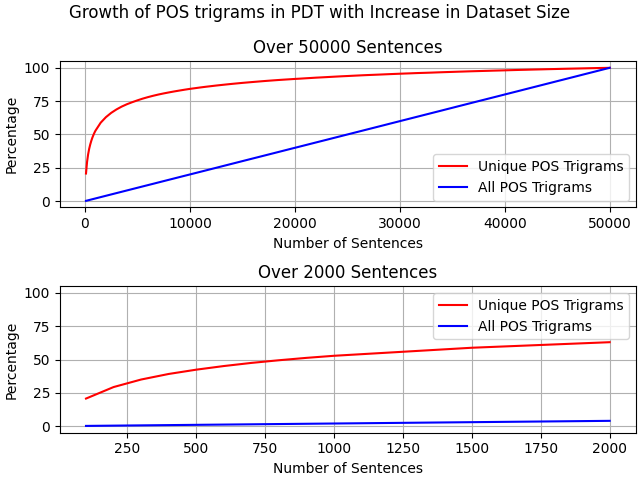
\includegraphics[scale=0.75]{img/trigram-stats-PDT.png}
    \caption{Growth of POS Trigrams in PDT with Increase in Dataset Size}
    \label{fig:trigram-PDT}
\end{figure}

\begin{figure}[H]
    \centering
    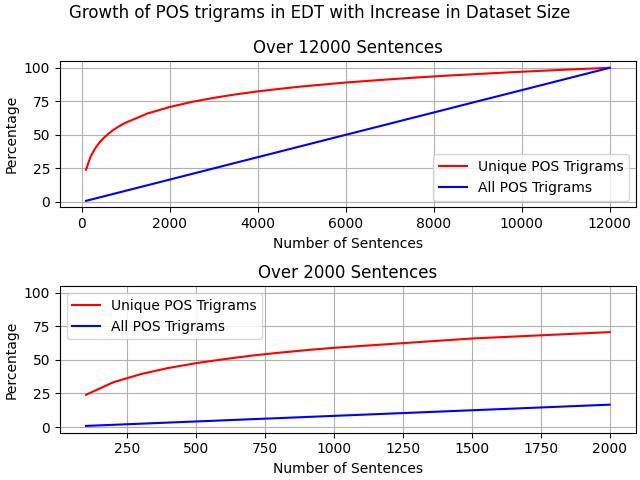
\includegraphics[scale=0.75]{img/trigram-stats-EDT.png}
    \caption{Growth of POS Trigrams in EDT with Increase in Dataset Size}
    \label{fig:trigram-EDT}
\end{figure}

As can be seen from the figures, the growth pattern is similar across both the languages. We can see that in case of a considerably small dataset size, the POS trigrams can not be considered as representative of those present in the entire dataset. We claim that for a proper estimation of the annotation consistency in two datasets belonging to the same genre, either dataset requires at least 400 sentences ($\approx 40\%$ of unique POS trigrams) for the estimation to be reliable. The minimum limitation on the size of the datasets ensures that the distribution of POS trigrams in either dataset is not skewed because of a small size.

\begin{claim}
Data across two datasets $A, B$ can be compared iff \\
\begin{equation*}
    \boxed{size(A) \geq 400 \And size(B) \geq 400}
\end{equation*}
\label{claim:pos_size_init}
\end{claim}

where $size(X)$ refers to the size of dataset $X$ in terms of the number of sentences

Table \ref{tab:counts-ar} shows the average sentence length of sentences in different treebanks for \verb|ar|. If we consider equal number of sentences from either of \verb|ar|-NYUAD or \verb|ar|-PADT treebanks and compare the POS annotation consistency with \verb|ar|-PUD treebanks, the total number of syntactic words differ by a factor of almost 2. 

\begin{table}[H]
    \centering
    \begin{tabular}{|l|l|l|l|}
    \hline
    \textbf{Counts} & \texttt{ar}-NYUAD & \texttt{ar}-PADT & \texttt{ar}-PUD \\
    \hline
    Syntactic Words & 738889 & 282384 & 20751 \\
    Sentences & 19738 & 7664 & 1000\\
    \hline
    \textbf{Average} & 37.434 & 36.845 & 20.751\\
    \hline
    \end{tabular}
    \caption[Average Sentence Lengths in \texttt{ar} Treebanks]{Average Sentence Lengths in \texttt{ar} Treebanks. In \texttt{es}, the token \textbf{v\'amonos} (Let's go) is split into 2 syntactic words \textbf{vamos} (go-\textit{1P-Pl.}) and \textbf{nos} (\textit{1P.-Pl.}) for annotation.}
    \label{tab:counts-ar}
\end{table}

When calculating the $\theta_{pos}$ scores for a set of treebanks, the average sentence length in either treebank should also be taken into account. It makes sense to limit the size of the datasets in consideration not in absolute terms, but also in reference to each other. Keeping this in mind, we update Claim \ref{claim:pos_size_init} to account for the average sentence length in Claim \ref{claim:pos_size}.

\begin{claim}
Data across two datasets $A, B$ can be compared iff \\
\begin{equation}
\label{eqn:size_constraint}
    \boxed{size(A) \geq 400 \And Avg(A) \geq Avg(B) \implies size(B) \cdot \frac{Avg(B)}{Avg(A)} \geq 400}
\end{equation}
\label{claim:pos_size}
\end{claim}

where 
\begin{enumerate}
    \item $Avg(X) = \frac{Total Syntactic Words(X)}{size(X)}$ is the average sentence length in dataset $X$
    \item $size(X)$ refers to the number of sentences in dataset $X$
\end{enumerate}

From the results of the data in Table \ref{tab:pos-harmony-size}, when the test split is composed of 500 instances ($k=100$ for \texttt{cs}; $k=24$ for \texttt{et}), the $\theta_{pos}$ metric is $\approx 0.3$. Considering that the larger $k$-values in either dataset do not satisfy the condition in Equation \ref{eqn:size_constraint}, we use the values as per the aforementioned $k$-values to estimate the maximal value for $\theta_{pos}$ when there is a size variance in the datasets.

As mentioned earlier, the treebanks in the consideration are ranked high in their quality check. Considering that some treebanks might not have such high quality of annotation, we allow some room for the change in $\theta_{pos}$ metric. 

If the datasets $A$, $B$ contain data from the same genre, and the size of the datasets is comparable (as per Equation \ref{eqn:size_constraint}), the upper limit on the $\theta_{pos}$ score can be specified as per Equation \ref{eqn:theta_pos_size_limit}.

\begin{equation}
    \boxed{\theta_{pos}(A,B) \leq \Theta_{pos}(A,B) = 0.5}
\label{eqn:theta_pos_size_limit}
\end{equation}

\section{Genre Distribution and \texorpdfstring{$\theta_{pos}$}{theta\_pos}}
\label{sec:pos-harmony-genre}

There can be significant difference(s) between genres in terms of syntactic annotations that are typical of the genre. While this difference is best exhibited across treebanks containing data from different genres, it can also be exhibited within a given treebank. The problem of music genre classification in speech data has been studied in detail, with different audio similarity metrics being proposed as well (cf. \cite{music1, music2}, among others). In the written data, while there has been some research on the study of inter-genre variations for language acquisition \citep{genre-acquisition1}, the classification of genres in textual corpus is identified mainly by the source of data.

\subsection{Relevant Literature on Textual Genres and Their Similarity}

In \cite{biber2}, a line of distinction is drawn between between text type and genre as the basis of classification of texts. While the former is `defined and distinguished on the basis of systematic nonlinguistic criteria', the latter is `defined on the basis of strictly linguistic criteria (similarities in the use of cooccuring linguistic features)' \cite[p.~39]{biber2}. In \cite{biber}, the different genres in \verb|en| are studied in different dimensions, focusing on one dimension at a time. The dimensions are a group of factors that associate the different features of a discourse, and are as listed in Table \ref{tab:dimensions-genres}. In the same work, the author notes that a given genre can contain multiple sub-genres which may or may not be internally coherent to each other \cite[p.~170]{biber}, and that no dimension in itself can attribute to the similarity or dissimilarity of the genres. In a later study that seeked to understand the variations of the genres based on these identified dimensions across 4 languages, the author notes that `even when defined at a high level of generality, parallel registers are more similar cross-linguistically than are disparate registers within a single language' \cite[p.~279]{biberbook}.

\begin{table}[H]
    \scalebox{0.9}{\begin{tabular}{|c|l|l|}
    \hline
    \textbf{S.No.} & \textbf{Dimension Name} & \textbf{Characteristic of Dimension} \\
    \hline
    \hline
    1. & \textbf{Involved vs Informational Production} & interactional, affective, involved \\
     & & purposes, associated with \\
     & & strict real-time production and \\
     & & comprehension constraints\\
    \hline
    2. & Narrative vs Non-Narrative Concerns & primary narrative purpose\\
    \hline
    3. & \textbf{Explicit vs Situation-Dependent} & identifies referents fully and \\
     & \textbf{Reference} & explicitly through relativization\\
    \hline
    4. & Overt Expression of Persuasion & speaker's expression of own \\
     & & point of view or with\\
     & & argumentative styles \\
     & & to persuade the addressee\\
    \hline
    5. & Abstract vs Non-Abstract Information & highly abstract and technical \\
    & & informational focus\\
    \hline
    6. & \textbf{On-Line Information Elaboration} & production under highly \\
    & & constrained conditions where \\
    & & information is presented \\
    & & in relatively loose, fragmented\\
    & & manner\\
    \hline
    \end{tabular}}
    \caption[Identified Dimensions for Comparison of Genres in \cite{biber}]{Identified Dimensions for Comparison of Genres. The characteristic of individual dimensions is as found in \cite[p.~115]{biber}. Dimension 5 on `Abstract vs Non-Abstract Information' is noted to be not universal across all languages \cite[p.~278]{biberbook}}
    \label{tab:dimensions-genres}
\end{table}

The dimensions marked in bold in Table \ref{tab:dimensions-genres} can be summarised under the notion of \textit{deep formality}, as coined in \cite{formality1}. \citeauthor{formality1} are able to classify linguistic constructions into different genres according to the measurement of their formality, based on a numerical measure of formality. The formality of a construction was numerically calculated in terms of F-measure (formality measure), as defined in Equation \ref{eqn:formality}. \cite{formality2} discovered that a numerical I-measure (informality measure, needed for working with Web2.0 data, given in Equation \ref{eqn:informality}) combined with F-measure worked better in identification of formality levels in data than when either of the measure was used on its own.

\begin{align}
    \text{F-measure} &= \textstyle{\frac{f_{noun} + f_{adjective} + f_{preposition} + f_{article} - f_{pronoun} - f_{verb} - f_{adverb} - f_{interjection} + 100}{2}} \label{eqn:formality}\\
    \text{I-measure} &= (f_{mistyped} + f_{interjection} + f_{emoticon}) * 100 \label{eqn:informality}
\end{align}
where $f_{A}$ represents relative frequency of $A$.

\subsection{Inter-Genre Similarity}

In our attempt at trying to understand the differences between different genres, we use F-measure as a primary classifying measure. Considering that CoNLL-U format does not differentiate between typos and other errors from the usual annotation in POS annotation\footnote{https://universaldependencies.org/u/overview/typos.html}, we do not use I-measure in our experiment.
% \newpage